\documentclass{article}
\usepackage[utf8]{inputenc}
\usepackage{polski}
\usepackage{graphicx}

\title{Mrówka Langtona}
\author{Jakub Przygodzki Adam Suski Grupa 1}
\date{Kwiecień 2018}

\begin{document}

\maketitle
\tableofcontents 

\newpage

\section{Wprowadzenie}
Napisany przez nas program symuluje mrówka Langtona. Jest to prosty automat komórkowy wymyślony i opisany przez Chrisa Langtona w 1986 roku. W każdym kroku wyróżniona jest jedna komórka nazywana "mrówką", która oprócz koloru ma określony także kierunek, w którym się porusza. Mrówka zachowuje się według następujących zasad:
\newline 1.   jeśli znajduje się na polu białym to obraca się w lewo (o kąt prosty), zmienia kolor pola na czarny i przechodzi na następną komórkę;
\newline  2.  jeśli znajduje się na polu czarnym to obraca się w prawo (o kąt prosty), zmienia kolor pola na biały i przechodzi na następną komórkę; 
\newline 3.  porusza się na nieskończonej planszy podzielonej na kwadratowe komórki (pola) w dwóch możliwych kolorach: czarnym i białym.

 
\section{Założenia początkowe}
Program został napisany jako model mrówki Langtona. Zostały nałożone pewne ograniczenia. 
\newline Liczba mrówek nie może byc większa od 5.
\newline Rozmiar planszy nie może byc większy niż 181 pól.
\newline Dla ułatwienia kazda mrówka ma swój kolor zadany przez twórców kodu.
\newline Maksymalny odstęp między wyswietlanymi ruchami mrówek wynosi 4 sekundy (za długo trzeba czekac na poszczególne ruchy mrówek).
\subsection{Plik konfiguracyjny}  Wymagane jest stworzenie pliku konfiguracyjnego. Jest on dostarczany do pragramu jako argument linii poleceń. Poszczególne dane w pliku konfiguracyjnym są rozdzielone spacjami.
\newline Pierwszy wiersz zawiera informacje o ilości mrówek, rozmiarze planszy po jakiej te mrówki się poruszają (rzeczywista liczba pól to liczba podana - 1) oraz czas odsepu pomiędzy wykonaniem się poszczególnych przesunięc mrówek. 
\newline Każdy i-ty wiersz zawiera informacje o i-1 mrówce (2 wiersz pliku zawiera informacje o 1 mrówce, itd.). Pierwsza liczba określa współrzędną x-ową mrówki na planszy, druga jej współrzędną y-kową. Trzecia liczba mówi o tym czy mrówka porusza się sposobem RL (2) czy LR (3). Ostatnia i czwarta liczba charakteryzuje kierunek, w którym skierowana jest mrówka (4 oznacza góra, 5 prawo, 6 dół, 7 lewo). 

\begin{figure}[ht]
\centering
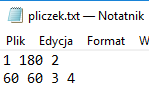
\includegraphics[scale=0.8]{plikKonfiguracyjny1}
\caption{Przykład poprawnego pliku konfiguracyjnego}
\label{fig:plikKonfiguracyjny1}
\end{figure}

\begin{figure}[ht]
\centering
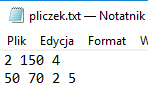
\includegraphics[scale=0.8]{plikKonfiguracyjny2}
\caption{Przykład niepoprawnego pliku konfiguracyjnego}
\label{fig:plikKonfiguracyjny2}
\end{figure}

Zakładamy, że podane przez użytkownika cechy mrówki tzn. liczby z odpowiedniego zakresu (np. użytkownik nie ustawi współrzędnej mrówki poza rozmiarem planszy). 
\newpage
\subsection{Biblioteka graficzna}
Do poprawnego działania programu wymagane jest zainstalowanie dodatkowej biblioteki graficznej SDL2. Przykład poprawnie skonfigurowanego IDE (w tym przypadku Code::Blocks 17.12).
\newline W folderze z projektem należy zamieścić plik SDL2.dll. Dodatkowo w opcjach linkowania nalezy wpisać -lmingw32 -lSDL2main -SDL2. 

\begin{figure}[h!]
\centering
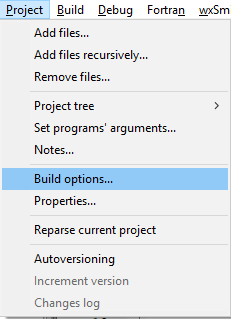
\includegraphics[scale=0.5]{projectBuildOptions}
\caption{Otwarte podmenu Project z zaznaczoną opcją, którą należy wybrać w celu skonfigurowania Build Options}
\label{fig:projectBuildOptions}
\end{figure}

\begin{figure}[ht]
\centering
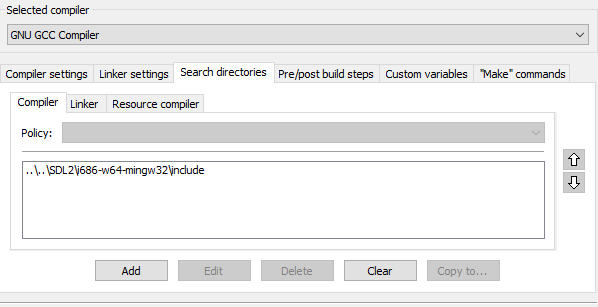
\includegraphics[scale=0.4]{include}
\caption{Compiler}
\label{fig:include}
\end{figure}

\begin{figure}[ht]
\centering
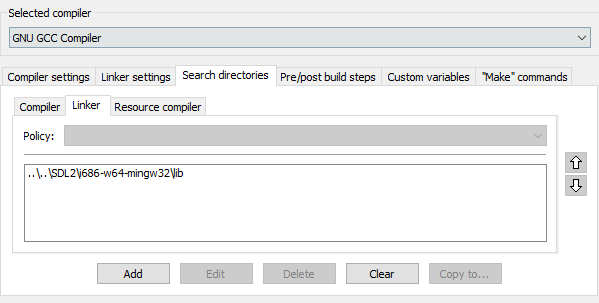
\includegraphics[scale=0.4]{lib}
\caption{Linker}
\label{fig:lib}
\end{figure}



\newpage

\section{Opis programu}
Program został stworzony z 4 modułów:
\newline 1) main - główny moduł,
\newline 2) board - moduł odpowiedzialny za tworzenie planszy po której poruszają się mrówki,
\newline 3) antt - moduł odpowiedzialny za poruszanie mrówek,
\newline 4) displaySDL - moduł odpowiedzialny za oprawę graficzną.

\subsection{main}
Główna funkcja programu ma za zadanie zczytać wszytskie dane z pliku konfiguracyjnego (antAmount - liczba mrówek, boardSize - rozmiar planszy, milisec - czas pomiędzy kolejneymi krokami algorytmu mrówki). 
\newline makeAnts() oraz antsAlgorithm() funkcje z modułu antt. boardGenrate() funkcja z modułu board.

\subsection{board}
Zawiera tylko jedną funkcję, która zwraca tablicę dwuwymiarową (a włąściwie wskaźnik na wskaźniki). Jako parametr przyjmuje integer czyli rozmiar planszy po, któej poruszają się mrówki (może ona mieć tylko wymiar kwadratowy). 
\newline int** boardGenerate( int x )
\newline Funkcja przyjmuje jako parametr zmienną x, która oznacza długość boku planszy.
\newline Zwracana jest macierz, która symbolizuje planszę, po której poruszają się mrówki, z wartością każdej komórki równej 0.
\newline

\subsection{antt}
Zdefiniowane pewne stałe w celu zwiększenia przejzystości i lepszemu zrozumieniu algorytmu.
\newline \#define ACTIVEA 1
\newline \#define NONACTIVEA 0
\newline \#define righth 2 
\newline \#define lefth 3 
\newline \#define N 4
\newline \#define E 5
\newline \#define S 6
\newline \#define W 7
\newline W stałych programowych ACTIVEA i NONACTIVEA literka A na końcu obydwu wyrazów oznacza ant. 
\newline
\newline
Struktura, która zawiera informacje o mrówkach.
\newline    x współrzędna x mrówki.
\newline     y współrzędna y mrówki.
\newline     handling zawiera informacje o aktualnym sterowaniu mrówki.
\newline     handlingOriginal zawiera informacje o pierwotnym sterowaniu mrówki(czy zaczyna od R czy L).
\newline     handlingDerivate jest przeczywieństwem handlingOriginal.
\newline     direction określa kierunek mrówki(góra, dół, prawo, lewo).
\newline
\newline typedef struct ant\{
\newline    int x, y, handling, handlingOriginal, handlingDerivate, direction;
\newline\};
\newline Został stworzony wskaźnik na tę strukturę, żeby łatwiej przechowywało informacje o kilku mrówkach.
\newline
\newline ants\_t makeAnts( int );
\newline Tworzy tablicę mrówek o rozmiarze zadanym przez użytkownika.
\newpage
int checkActivity( ants\_t, int i, int );
\newline Sprawdza aktywność (czy znajduje się na planszy i -tej mrówki). Jako trzeci parametr podany jest rozmair planszy. Zwraca 1 jeśli mrówka jest aktywna (na planszy), 0 w przeciwnym wypadku.
\newline
\newline
\newline void changePosition( ants\_t, int i );
\newline Zmienia pozycję i-tej mrówki. Zasada działania jest zgodna z algorytmem mrówki dal 2 możliwości poruszani (RL i LR).
\newline
\newline void antsAlgorithm( int**, int, ants t, int, int );
\newline Zasadniczy algorytm poruszania mrówkami. Zmienia sterowanie zależnie od pozycji w jakiej znajduje się mróka, następnie wywołuje funkcję changePosition() i checkActivity() dla każdej mrówki. W między czasie zlicza ilość aktywnych mrówek. Po wykonaniu skoku każdej z mrówek, wyświetla aktualny stan planszy (antShow()). Jeśli, któa kolwiek mrówka jest już nieaktywna, bądź użytkownik nacisnął przycisk zamknięcia okna praca z programem się kończy.    

\newpage
\subsection{displaySDL}
\#include "SDL2/SDL.h"
\newline Określony rozmiar mrówki, który pozwala we względnie wygodny sposób obserwować ruch mrówki.
\newline \#define ANTSIZE 4
\newline Window* window;
\newline Renderer* renderer;
\newline SDL Rect ant;
\newline 
\newline void drawBlack( int xm, int ym );
\newline Zamalowywuje komórke napotkaną przez mrówkę z powrotem na czarno.
\newline     xm współrzędna x mrówki.
\newline     ym współrzędna y mrówki.
\newline
\newline void drawColor( int xm, int ym , int i );
\newline    Zamalowywuje komórke napotkaną przez i-tą mrówkę na odpowiadający jej kolor.
\newline     xm współrzędna x mrówki.
\newline     ym współrzędna y mrówki.
\newline
\newline int initEverything( int boardSize );
\newline Inicjalizuje pracę SDL
\newline    Zwraca 1 jeśli uda się zacząć pracę z SDL, w przeciwnym wypadku zwraca 0.
\newline
\newline void destroymySDL();
\newline 
    Kończy pracę z SDL.
\newline 
\newline void antShow( int delay );
\newline Odpowiada za wywołanie rendera oraz opóźnienia (delay) między wykonanymi krokami algorytmu mróki
\newpage
\section{Dane wyjściowe}
Po porawnym uruchomieniu programu ukazuje się ekran przedstawiający planszę po której poruszają się mrówki. Użytkownik zobaczy każde przejście po kolei, aż do osiągnięcia przez mrówkę granicy planszy lub naciśnięcia przez użytkownika przycisku zamknięcia okna.

\begin{figure}[ht]
\centering
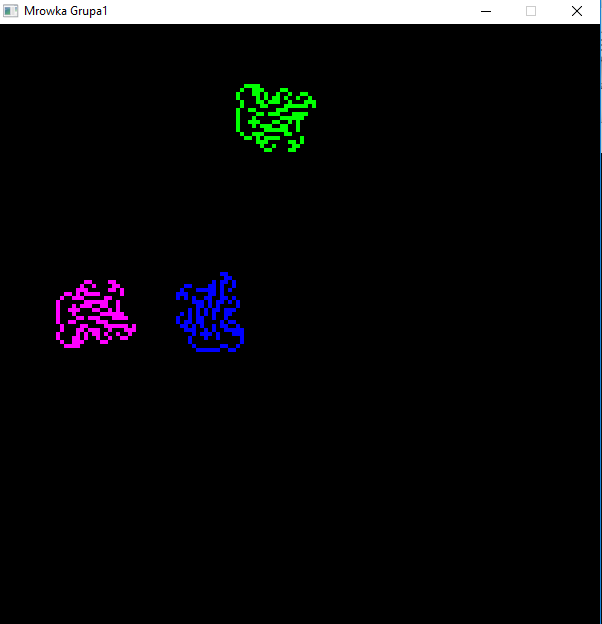
\includegraphics[scale=0.4]{przykladUruch}
\caption{Przykład uruchomienia programu}
\label{fig:przykladUruch}
\end{figure}

W przypadku nieprawidłowego uruchomienia programu (nie podanie lub błędny plik konfiguracyjny, nieodpowiednie dane wejściowe, itp.) zostanie wyświetlony odpoweidni komunikat o wystąpionym błędzie i program sie zakończy. 

\end{document}
